\chapter{Probability}


\section{Probability}
\begin{description}
    \item[State space] \marginnote{State space}
        Set $\Omega$ of all the possible results of an experiment.
        \begin{example}
            A coin is tossed two times. 
            $\Omega = \{ (\text{T}, \text{T}), (\text{T}, \text{H}), (\text{H}, \text{T}), (\text{H}, \text{H}) \}$
        \end{example}

    \item[Event] \marginnote{Event}
        Set of possible results (i.e. $A$ is an event if $A \subseteq \Omega$)

    \item[Probability] \marginnote{Probability}
        Let $\mathbb{E}$ be the set of all the possible events (i.e. power set of $\Omega$).
        The probability is a function:
        \[ \prob{A}: \mathbb{E} \rightarrow [0, 1] \]
        \begin{example}
            Let $\Omega$ be as above.
            Given an event $A = \{ (\text{T}, \text{H}), (\text{H}, \text{T}) \}$, 
            its probability is: $\prob{A} = \frac{2}{4} = \frac{1}{2}$
        \end{example}

    \item[Conditional probability] \marginnote{Conditional probability}
        Probability of an event $B$, knowing that another event $A$ happened:
        \[ \prob{B \vert A} = \frac{\prob{A \cap B}}{\prob{A}} \text{, with } \prob{A} \neq 0 \]

        \begin{example}
            A coin is tossed three times. 
            Given the events $A = \{ \text{tails two times} \}$ and $B = \{ \text{one heads and one tails} \}$
            We have that:

            \begin{minipage}{\linewidth}
                \centering
                \small
                $\Omega = \{ 
                    (\text{T}, \text{T}, \text{T}), (\text{T}, \text{T}, \text{H}), (\text{T}, \text{H}, \text{T})
                    (\text{T}, \text{H}, \text{H}), (\text{H}, \text{T}, \text{T}), (\text{H}, \text{T}, \text{H})
                    (\text{H}, \text{H}, \text{T}), (\text{H}, \text{H}, \text{H})
                \}$
            \end{minipage}

            \begin{minipage}{.325\linewidth}
                \centering
                $\prob{A} = \frac{4}{8} = \frac{1}{2}$
            \end{minipage}
            \begin{minipage}{.325\linewidth}
                \centering
                $\prob{B} = \frac{6}{8} = \frac{3}{4}$
            \end{minipage}
            \begin{minipage}{.325\linewidth}
                \centering
                $\prob{A \cap B} = \frac{3}{8}$
            \end{minipage}

            \begin{minipage}{.48\linewidth}
                \centering
                $\prob{A \vert B} = \frac{3/8}{3/4} = \frac{1}{2}$
            \end{minipage}
            \begin{minipage}{.48\linewidth}
                \centering
                $\prob{B \vert A} = \frac{3/8}{1/2} = \frac{3}{4}$
            \end{minipage}
        \end{example}

    \item[Independent events] \marginnote{Independent events}
        Two events $A$ and $B$ are independent if:
        \[ \prob{A \cap B} = \prob{A}\prob{B} \]
        It follows that:

        \begin{minipage}{.48\linewidth}
            \centering
            $\prob{A \vert B} = \prob{A}$
        \end{minipage}
        \begin{minipage}{.48\linewidth}
            \centering
            $\prob{B \vert A} = \prob{B}$
        \end{minipage}

        In general, given $n$ events $A_1, \dots, A_n$, they are independent if:
        \[ \prob{A_1 \cap \dots \cap A_n} = \prod_{i=1}^{n} \prob{A_i} \]
\end{description}



\section{Random variables}
\begin{description}
    \item[Random variable (RV)] \marginnote{Random variable}
        A random variable $X$ is a function:
        \[ X: \Omega \rightarrow \mathbb{R} \]

    \item[Target space/Support] \marginnote{Target space}
        Given a random variable $X$, 
        the target space (or support) $\mathcal{T}_X$ of $X$ is the set of all its possible values:
        \[ \mathcal{T}_X = \{ x \mid x = X(\omega), \forall \omega \in \Omega \} \]
\end{description}


\subsection{Discrete random variables}

\begin{description}
    \item[Discrete random variable] \marginnote{Discrete random variable}
        A random variable $X$ is discrete if its target space $\mathcal{T}_X$ is finite or countably infinite.

        \begin{example}
            A coin is tossed twice.

            The random variable is $X(\omega) = \{ \text{number of heads} \}$.
            We have that $\mathcal{T}_X = \{ 0, 1, 2 \}$, therefore $X$ is discrete.
        \end{example}

        \begin{example}
            Roll a die until 6 comes out.

            The random variable is $Y(\omega) = \{ \text{number of rolls before 6} \}$.
            We have that $\mathcal{T}_Y = \{ 1, 2, \dots \} = \mathbb{N} \smallsetminus \{0\}$, 
            therefore $Y$ is discrete as $\mathcal{T}_Y$ is a countable set.
        \end{example}

    \item[Probability mass function (PMF)] \marginnote{Probability mass function (PMF)}
        Given a discrete random variable $X$, its probability mass function is a function $f_X: \mathcal{T}_X \rightarrow [0, 1]$ such that:
        \[ f_X(x) = \prob{X = x}, \forall x \in \mathcal{T}_X \]

        A PMF has the following properties:
        \begin{enumerate}
            \item $f_X(x) \geq 0, \forall x \in \mathcal{T}_X$
            \item $\sum_{x \in \mathcal{T}_X} f_X(x) = 1$
            \item Let $A \subseteq \Omega$, $\prob{X = x \in A} = \sum_{x \in A} f_X(x)$
        \end{enumerate}

        \begin{example}
            Let $\Omega = \{ (\text{T}, \text{T}), (\text{T}, \text{H}), (\text{H}, \text{T}), (\text{H}, \text{H}) \}$.
            Given a random variable $X = \{ \text{number of heads} \}$ with $\mathcal{T}_X = \{ 0, 1, 2 \}$.
            The PMF is:
            \[
                \begin{split}
                    f_X &= \prob{X = 0} = \frac{1}{4} \\
                    f_X &= \prob{X = 1} = \frac{2}{4} \\
                    f_X &= \prob{X = 2} = \frac{1}{4}
                \end{split}  
            \]
        \end{example}
\end{description}

\subsubsection{Common distributions}
\begin{descriptionlist}
    \item[Uniform distribution] \marginnote{Uniform distribution}
        Given a discrete random variable $X$ with $\#(\mathcal{T}_X) = N$,
        $X$ has an uniform distribution if:
        \[ f_X(x) = \frac{1}{N}, \forall x \in \mathcal{T}_X \]
    
    \item[Poisson distribution] \marginnote{Poisson distribution}
        Given a discrete random variable $X$ with mean $\lambda$,
        $X$ has a poisson distribution if:
        \[ f_X(x) = e^{-\lambda} \frac{\lambda^x}{x!}, \forall x \in \mathcal{T}_X \]
\end{descriptionlist}


\subsection{Continuous random variables}

\begin{description}
    \item[Continuous random variable] \marginnote{Continuous random variable}
        A random variable $X$ is continuous if its target space $\mathcal{T}_X$ is uncountably infinite (i.e. a subset of $\mathbb{R}$).
        Usually, $\mathcal{T}_X$ is an interval or union of intervals.

        \begin{example}
            Given a random variable $Z = \{ \text{Time before the arrival of a client} \}$.
            $Z$ is continuous as $\mathcal{T}_Z = [a, b] \subseteq [0, +\infty[$ is an uncountable set.
        \end{example}

    \item[Probability density function (PDF)] \marginnote{Probability density function (PDF)}
        Given a continuous random variable $X$, 
        its probability density function is a function $f_X: \mathcal{T}_X \rightarrow \mathbb{R}$ such that:
        \[ \prob{X \in A} = \int_{A} f_X(x) \,dx \]
        \[ \prob{a \leq X \leq b} = \int_{a}^{b} f_X(x) \,dx \]
        Note that $\prob{X = a} = \prob{a \leq X \leq a} = \int_{a}^{a} f_X(x) \,dx = 0$

        A PDF has the following properties:
        \begin{enumerate}
            \item $f_X(x) \geq 0, \forall x \in \mathcal{T}_X$ 
            \item $\int_{x \in  \mathcal{T}_X} f_X(x) \,dx = 1$
            \item $\prob{X \in A} =  \int_{A} f_X(x) \,dx$
        \end{enumerate}
\end{description}

\subsubsection{Common distributions}
\begin{descriptionlist}
    \item[Continuous uniform distribution] \marginnote{Continuous uniform distribution}
        Given a continuous random variable $X$ with $\mathcal{T}_X = [a, b]$,
        $X$ has a continuous uniform distribution if:
        \[ f_X(x) = \frac{1}{b-a}, \forall x \in \mathcal{T}_X \]
    
    \item[Normal distribution] \marginnote{Normal distribution}
        Given a continuous random variable $X$ and the parameters $\mu$ (mean) and $\sigma$ (variance).
        $X$ has a normal distribution if:
        \[ f_X(x) = \frac{1}{\sigma \sqrt{2\pi}} e^{\frac{-(x-\mu)^2}{2\sigma^2}} , \forall x \in \mathcal{T}_X\]

        \begin{description}
            \item[Standard normal distribution] \marginnote{Standard normal distribution}
                Normal distribution with $\mu = 0$ and $\sigma = 1$.
        \end{description}

        \begin{figure}[ht]
            \centering
            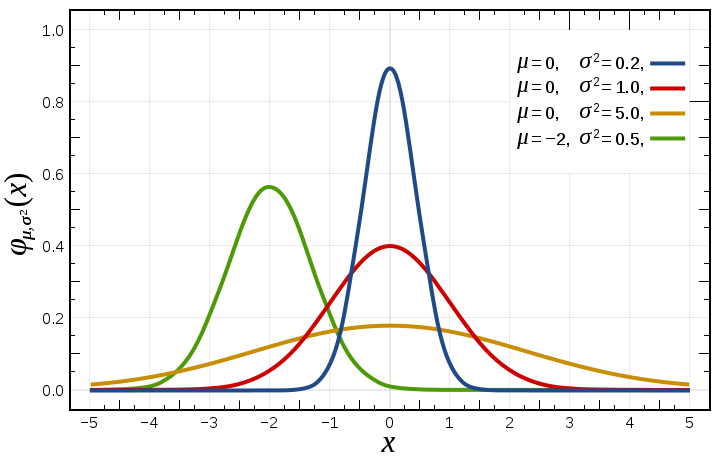
\includegraphics[width=0.5\textwidth]{img/normal_distribution.png}
            \caption{Normal distributions and standard normal distribution}
        \end{figure}
\end{descriptionlist}